\section{Architecture overview}

  \begin{figure}[h!]
      \centering
      \vspace{1em}
\scalebox{0.75}{
\begin{tikzpicture}[scale=1.25, draw=gray, inner sep=0, outer sep=0]
  \node[rectangle, draw=black,
    minimum height = 1.25cm,
    minimum width = 13cm,
    fill = gray!20] (EMM) at (7.5, -2.5) {EMM};
  \node[rectangle, draw=black,
    minimum height = 2cm,
    minimum width = 2cm,
    fill = blue!30!gray!20] (IFM) at (3, 0) {IFM};
  \node[rectangle, draw=black,
    minimum height = 2cm,
    minimum width = 2cm,
    fill = blue!30!gray!20] (DECM) at (6, 0) {DECM};
  \node[rectangle, draw=black,
    minimum height = 1.25cm,
    minimum width = 13cm,
    fill = gray!20] (REGM) at (10.5, 2.5) {REGM};
  \node[rectangle, draw=black,
    minimum height = 2cm,
    minimum width = 2cm,
    fill = blue!30!gray!20] (EXM) at (9, 0) {EXM};
  \node[rectangle, draw=black,
    minimum height = 2cm,
    minimum width = 2cm,
    fill = blue!30!gray!20] (LSM) at (12, 0) {LSM};
  \node[rectangle, draw=black,
    minimum height = 2cm,
    minimum width = 2cm,
    fill = blue!30!gray!20] (WBM) at (15, 0) {WBM};
  \node[rectangle, draw=red,
    anchor=north east,
    minimum height = 1.25cm,
    minimum width = 2cm,
    fill = red!20] (HZDM) at ([xshift=-1.25cm]REGM.north west) {HZDM};

  \node (hzdm-port1) at ([xshift=-0.4cm]HZDM.south) {};
  \node (hzdm-port2) at ([xshift=-0.2cm]HZDM.south) {};
  \node (hzdm-port3) at ([xshift=0.0cm]HZDM.south) {};
  \node (hzdm-port4) at ([xshift=0.2cm]HZDM.south) {};
  \node (hzdm-port5) at ([xshift=0.4cm]HZDM.south) {};
  \node (ifm-hzd-port) at (IFM.north) {};
  \node (decm-hzd-port) at ([xshift=-0.4cm]DECM.north) {};
  \node (decm-hzd-port-mid) at ([yshift=0.3cm]decm-hzd-port.center) {};
  \node (exm-hzd-port) at ([xshift=-0.4cm]EXM.north) {};
  \node (exm-hzd-port-mid) at ([yshift=0.5cm]exm-hzd-port.center) {};
  \node (lsm-hzd-port) at ([xshift=-0.4cm]LSM.north) {};
  \node (lsm-hzd-port-mid) at ([yshift=0.7cm]lsm-hzd-port.center) {};
  \node (wbm-hzd-port) at ([xshift=-0.4cm]WBM.north) {};
  \node (wbm-hzd-port-mid) at ([yshift=0.9cm]wbm-hzd-port.center) {};
  \draw[-, red] (hzdm-port1 |- ifm-hzd-port) -- (hzdm-port1);
  \draw[-, red] (decm-hzd-port) -- (decm-hzd-port-mid) -- (hzdm-port2 |- decm-hzd-port-mid) -- (hzdm-port2);
  \draw[-, red] (exm-hzd-port) -- (exm-hzd-port-mid) -- (hzdm-port3 |- exm-hzd-port-mid) -- (hzdm-port3);
  \draw[-, red] (lsm-hzd-port) -- (lsm-hzd-port-mid) -- (hzdm-port4 |- lsm-hzd-port-mid) -- (hzdm-port4);
  \draw[-, red] (wbm-hzd-port) -- (wbm-hzd-port-mid) -- (hzdm-port5 |- wbm-hzd-port-mid) -- (hzdm-port5);

  \draw[->] (IFM.east) -- (DECM.west);
  \draw[->] (DECM.east) -- (EXM.west);
  \draw[->] (EXM.east) -- (LSM.west);
  \draw[->] (LSM.east) -- (WBM.west);

  \draw[<-] (IFM.south) -- (IFM.south|- EMM.north);

  \draw[->] ([xshift=-0.25cm]LSM.south) -- ([xshift=-0.25cm]LSM.south |- EMM.north);
  \draw[<-] ([xshift=0.25cm]LSM.south) -- ([xshift=0.25cm]LSM.south |- EMM.north);

  \draw[<-] (DECM.north) -- (DECM.north |- REGM.south);
  \draw[->] (WBM.north) -- (WBM.north |- REGM.south);

  % surrounding rectangle
  \node[dashed, draw=black, align=center, inner sep=0.5cm, fit=(HZDM) (EMM) (IFM) (DECM) (EXM) (WBM) (REGM)] (border) {};

  % external interface
  \node (irq) at ([yshift=0.25cm]IFM.west) {};
  \node (drq) at ([yshift=-0.25cm]IFM.west) {};
  \node (axi) at (EMM.west) {};
  \node (clk) at ([yshift=-1.25cm]border.north west) {};
  \node (rst) at ([yshift=-1.75cm]border.north west) {};

  \node (extend) at ([xshift=-1.5cm]irq.center) {};

  \draw[->] (clk.center -| extend.center) node[left=0.2cm, anchor=east]{\small CLK} -- (clk.center);
  \draw[->] (rst.center -| extend.center) node[left=0.2cm, anchor=east]{\small RST\_N} -- (rst.center);
  \draw[->] (irq.center -| extend.center) node[left=0.2cm, anchor=east]{\small IRQ} -- (irq.center);
  \draw[->] (drq.center -| extend.center) node[left=0.2cm, anchor=east]{\small DRQ} -- (drq.center);
  \draw[<->, thick] (axi.center -| extend.center) node[left=0.2cm, anchor=east]{\small Wishbone} -- (axi.center);

  % clk triangle
  \draw[-, dashed, draw=black] ([yshift=0.25cm]clk.center) -- ([xshift=0.25cm]clk.center) -- ([yshift=-0.25cm]clk.center);

  % branch unit
  \draw[->] ([yshift=-0.25cm]EXM.west) -- ([xshift=-0.5cm, yshift=-0.25cm]EXM.west) -- ([xshift=-0.5cm, yshift=-1.25cm]EXM.west) -- node[below=0.2cm]{\footnotesize Branch} ([xshift=0.5cm, yshift=-1.25cm]IFM.east) -- ([xshift=0.5cm, yshift=-0.25cm]IFM.east) -- ([yshift=-0.25cm]IFM.east);

\end{tikzpicture}
}

      \caption{Schematic view of the architecture of ECAP5-DPROC}
      \label{fig:architecture}
    \end{figure}

  \subsection{Clock domains}

    \begin{content}
        To simplify the design of revision 1.0.0, each module of ECAP5-DPROC belong to a unique clock domain.
      \end{content}

  \subsection{Pipeline stages}

    \begin{content}
        ECAP5-DPROC is built around a pipelined architecture with the following stages :
        \begin{itemize}
            \item The instruction fetch stage loads the next instruction from memory.
            \item The decode stage handles the instruction decoding to provide the next stage with the different instruction input values including reading from internal registers.
            \item The execute stage implements all arithmetic and logic operations. This includes load and store operations to the memory.
            \item The write-back stage which handles storing instructions outputs to internal registers.
          \end{itemize}
        Considering the load-store architecture of the RISC-V instruction set, the choice was made, for revision 1.0.0, to include the memory stage of the typical 5-stage pipeline within the execute stage. This will decrease the latency while keeping a similar throughput, as any memory access will inevitably produce a pipeline stall as of revision 1.0.0.
      \end{content}

    \subsubsection{Pipeline stall}

      \label{pipeline-stall}

      \begin{content}
          In order to handle pipeline stalls, a handshaking mechanism is implemented between each stages, allowing the execution flow to be stopped. A stall can be either triggered by a stage itself or requested by the hazard module.
        \end{content}

      \begin{figure}[H]
          \centering
          \scalebox{1}{
\begin{tikzpicture}[->, >=stealth, node distance=4cm, every state/.style={thick, fill=gray!20}, initial text=$ $]
    \node[state] (q1) at (0, 0) {\small stall};
    \node[state, accepting] (q2) at (3, 0) {\small normal};
    \node[state] (q3) at (6, 2) {\small bubble};
    \node[state] (q4) at (6, -2) {\small wait};
    \draw   (q1) edge[bend left, above=2cm] node{\footnotesize{b}} (q2)
            (q2) edge[bend left, below=2cm] node{\footnotesize{a}} (q1)
            (q2) edge[bend left, above=3cm] node{\footnotesize{c}} (q3)
            (q3) edge[bend left, below=2cm] node{\footnotesize{d}} (q2)
            (q2) edge[bend left, above=2cm] node{\footnotesize{e}} (q4)
            (q4) edge[bend left, below=2cm] node{\footnotesize{f}} (q2);
\end{tikzpicture}
}
\vspace{1em}
\begin{center}
  \scriptsize \textit{a : stage stalls, }
  \scriptsize \textit{b : stage unstalls, }
  \scriptsize \textit{c : input valid = 0, }
  \scriptsize \textit{d : input valid = 1, }
  \scriptsize \textit{e : output ready = 0, }
  \scriptsize \textit{f : output valid = 1, }
\end{center}
          \caption{State diagram of the operating modes of pipeline stages}
          \label{fig:pipeline-stage-state}
        \end{figure}

      \begin{content}
          Pipeline stages located at the start and end of the pipeline do not implement the bubble and wait modes respectively.
          
          The following points describe the behavior of the different modes :
          \begin{itemize}
              \item A stage in \textbf{normal} mode shall operate as described by its different functional behaviors.
              \item A stage in \textbf{stall} mode shall deassert its input ready signal and output valid signal while waiting to unstall.
              \item A stage in \textbf{bubble} mode shall operate as normal but taking a nop instruction as input instead of the data provided by the preceding stage.
              \item A stage in \textbf{wait} mode shall deassert its input ready signal and wait until going back to normal mode.
            \end{itemize}
          
          In case of a stall, the stalling stage deasserts its input ready signal leading to preceding stages waiting for completion. The stalling stage deasserts its output valid signal leading to following stages taking a bubble as their input.

          The figure \ref{fig:pipeline-behavior-wait-stall} is a diagram of the stall behavior on a 5-stage pipeline. By stalling the 3\textsuperscript{rd} stage, this example provides a representative visualisation of all the stalling cases of a 4-stage pipeline.
        \end{content}

      \begin{figure}[H]
          \centering
          \vspace{1em}
\scalebox{0.85}{
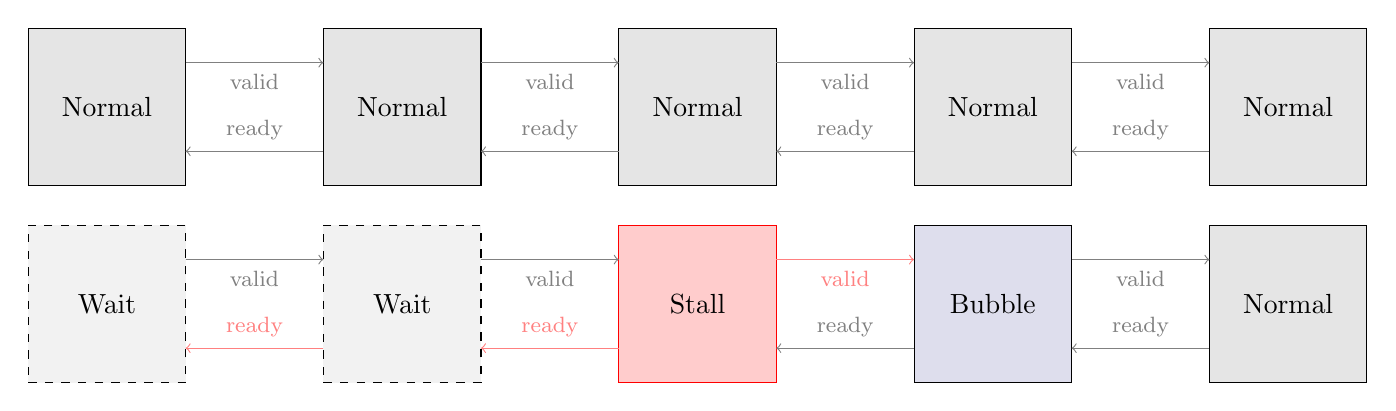
\begin{tikzpicture}[scale=1.25, draw=gray, inner sep=0, outer sep=0]
% STEP 1
  \node[rectangle, draw=black,
    align=center,
    minimum height = 2cm,
    minimum width = 2cm,
    fill = gray!20] (stage3_1) at (0, 0) {Normal};
  \node[rectangle, draw=black,
    align=center,
    minimum height = 2cm,
    minimum width = 2cm,
    fill = gray!20] (stage2_1) at (-3, 0) {Normal};
  \node[rectangle, draw=black,
    align=center,
    minimum height = 2cm,
    minimum width = 2cm,
    fill = gray!20] (stage1_1) at (-6, 0) {Normal};
  \node[rectangle, draw=black,
    align=center,
    minimum height = 2cm,
    minimum width = 2cm,
    fill = gray!20] (stage4_1) at (3, 0) {Normal};
  \node[rectangle, draw=black,
    align=center,
    minimum height = 2cm,
    minimum width = 2cm,
    fill = gray!20] (stage5_1) at (6, 0) {Normal};

  \draw[->] ([yshift=0.45cm]stage1_1.east)  -- node[text=gray, below=0.15cm]{\footnotesize{valid}} ([yshift=0.45cm]stage2_1.west);
  \draw[<-] ([yshift=-0.45cm]stage1_1.east) -- node[text=gray, above=0.15cm]{\footnotesize{ready}} ([yshift=-0.45cm]stage2_1.west);

  \draw[->] ([yshift=0.45cm]stage2_1.east) -- node[text=gray, below=0.15cm]{\footnotesize{valid}} ([yshift=0.45cm]stage3_1.west);
  \draw[<-] ([yshift=-0.45cm]stage2_1.east) -- node[text=gray, above=0.15cm]{\footnotesize{ready}} ([yshift=-0.45cm]stage3_1.west);

  \draw[->] ([yshift=0.45cm]stage3_1.east) -- node[text=gray, below=0.15cm]{\footnotesize{valid}} ([yshift=0.45cm]stage4_1.west);
  \draw[<-] ([yshift=-0.45cm]stage3_1.east) -- node[text=gray, above=0.15cm]{\footnotesize{ready}} ([yshift=-0.45cm]stage4_1.west);

  \draw[->] ([yshift=0.45cm]stage4_1.east) -- node[text=gray, below=0.15cm]{\footnotesize{valid}} ([yshift=0.45cm]stage5_1.west);
  \draw[<-] ([yshift=-0.45cm]stage4_1.east) -- node[text=gray, above=0.15cm]{\footnotesize{ready}} ([yshift=-0.45cm]stage5_1.west);

% STEP 2
  \node[rectangle, draw=red,
    align=center,
    minimum height = 2cm,
    minimum width = 2cm,
    fill = red!20] (stage3_2) at (0, -2) {Stall};
  \node[dashed, rectangle, draw=black,
    align=center,
    minimum height = 2cm,
    minimum width = 2cm,
    fill = gray!10] (stage2_2) at (-3, -2) {Wait};
  \node[dashed, rectangle, draw=black,
    align=center,
    minimum height = 2cm,
    minimum width = 2cm,
    fill = gray!10] (stage1_2) at (-6, -2) {Wait};
  \node[rectangle, draw=black,
    align=center,
    minimum height = 2cm,
    minimum width = 2cm,
    fill = blue!30!gray!20] (stage4_2) at (3, -2) {Bubble};
  \node[rectangle, draw=black,
    align=center,
    minimum height = 2cm,
    minimum width = 2cm,
    fill = gray!20] (stage5_2) at (6, -2) {Normal};

  \draw[->] ([yshift=0.45cm]stage1_2.east)  -- node[text=gray, below=0.15cm]{\footnotesize{valid}} ([yshift=0.45cm]stage2_2.west);
  \draw[<-, red!50] ([yshift=-0.45cm]stage1_2.east) -- node[text=red!50, above=0.15cm]{\footnotesize{ready}} ([yshift=-0.45cm]stage2_2.west);

      \draw[->] ([yshift=0.45cm]stage2_2.east) -- node[text=gray, below=0.15cm]{\footnotesize{valid}} ([yshift=0.45cm]stage3_2.west);
  \draw[<-, red!50] ([yshift=-0.45cm]stage2_2.east) -- node[text=red!50, above=0.15cm]{\footnotesize{ready}} ([yshift=-0.45cm]stage3_2.west);

  \draw[->, red!50] ([yshift=0.45cm]stage3_2.east) -- node[text=red!50, below=0.15cm]{\footnotesize{valid}} ([yshift=0.45cm]stage4_2.west);
  \draw[<-] ([yshift=-0.45cm]stage3_2.east) -- node[text=gray, above=0.15cm]{\footnotesize{ready}} ([yshift=-0.45cm]stage4_2.west);

  \draw[->] ([yshift=0.45cm]stage4_2.east) -- node[text=gray, below=0.15cm]{\footnotesize{valid}} ([yshift=0.45cm]stage5_2.west);
  \draw[<-] ([yshift=-0.45cm]stage4_2.east) -- node[text=gray, above=0.15cm]{\footnotesize{ready}} ([yshift=-0.45cm]stage5_2.west);
\end{tikzpicture}
}

          \caption{Diagram of a pipeline stall behavior on a 6-stage pipeline}
          \label{fig:pipeline-behavior-wait-stall}
        \end{figure}

      \begin{content}
          Figure \ref{fig:pipeline-behavior-wait-stall-resolution} outlines the resolution of a pipeline stall on stage 3. By stalling the 3\textsuperscript{rd} stage, this example provides a representative visualisation of all the stalling cases of a 4-stage pipeline.
        \end{content}

      \begin{figure}[H]
          \centering
          \makeatletter\gdef\dividers{}
\begin{tikztimingtable}[%
    scale=0.7,
    timing/dslope=0.1,
    timing/.style={x=5ex,y=3ex},
    x=5ex,
    timing/rowdist=4ex,
    timing/name/.style={font=\footnotesize},
    timing/u/background/.style={fill=gray!20},
    timing/e/background/.style={fill=gray!20},
]
clk\_i & H 7{C C} L \\
rst\_i & 2E 12L 2E\\
& \divider{Stage 1} \\
stage1\_instr         & 2U 2D{a} 2D{b} 6D{c}             2D{d} 2U \\
stage1\_output\_valid & 2.5E 2H    2H    2H    2H    2H    2H    1.5E \\
stage2\_input\_ready  & 2.5E 2H    2H    2L    2L    2H    2H    1.5E \\
& \divider{Stage 2} \\
stage2\_instr         & 2U 2U    2D{a} 6D{b}             2D{c} 2D{d} \\
stage2\_output\_valid & 2.5E 2H    2H    2H    2H    2H    2H    1.5H \\
stage3\_input\_ready  & 2.5E 2H    2H    2L    2L    2H    2H    1.5H \\
& \divider{Stage 3} \\
stage3\_instr         & 2U 2U    2U    6D{a}             2D{b} 2D{c} \\
stage3\_output\_valid & 2.5E 2H    2H    2L    2L    2H    2H    1.5H \\
stage4\_input\_ready  & 2.5E 2H    2H    2H    2H    2H    2H    1.5H \\
& \divider{Stage 4} \\
stage4\_instr         & 2U 2U    2U  2U  4D{nop}           2D{a} 2D{b} \\
stage4\_output\_valid & 2.5E 2H    2H    2H    2H    2H    2H    1.5H \\
stage5\_input\_ready  & 2.5E 2H    2H    2H    2H    2H    2H    1.5H \\
& \divider{Stage 5} \\
stage5\_instr         & 2U 2U    2U    2U  2U  4D{nop}           2D{a} \\
\extracode
% grid
\begin{pgfonlayer}{background}
\begin{scope}[semitransparent ,semithick]
\vertlines[darkgray,dotted]{2, 4, 6, 8, 10, 12, 14}

\draw[decorate, decoration = {brace, amplitude=5pt}] (2, 3.5) -- node[above=0.3cm]{\footnotesize{Normal}} (5.8, 3.5);
\draw[decorate, decoration = {brace, amplitude=5pt}] (6.2, 3.5) -- node[above=0.3cm]{\footnotesize{Stall}} (9.8, 3.5);
\draw[decorate, decoration = {brace, amplitude=5pt}] (10.2, 3.5) -- node[above=0.3cm]{\footnotesize{Normal}} (14, 3.5);

\dividers 
\end{scope}
\end{pgfonlayer}
\end{tikztimingtable}

          \caption{Timing diagram of a pipeline stall resolution behavior on a 6-stage pipeline}
          \label{fig:pipeline-behavior-wait-stall-resolution}
        \end{figure}

  \subsection{Hazard management}

    \subsubsection{Structural hazard}

      \begin{content}
          For the scope of this document, are designated as structural hazards all cases when a stage is unable to finish its processing within the required time before the next clock cycle.

          A pipeline stall is produced in case of structural hazards. It shall be noted that the some of the performance impact of this kind of hazard could be mitigated but this feature is not included in revision 1.0.0.
        \end{content}

    \subsubsection{Data hazard}

      \begin{content}
          A data hazard occurs when an instruction (A) uses the result of a previous instruction (B) which is still being processed in the pipeline.

          A pipeline stall is produced in case of data hazards so that B is able to finish before A uses its result. It shall be noted that some of the performance impact of this kind of hazard could be mitigated but this feature is not included in revision 1.0.0.
        \end{content}

    \subsubsection{Control hazard}

      \label{control-hazard}

      \begin{content}
          A control hazard occurs when a jump or branch instruction is executed, as instructions following the jump/branch are already being processes through the pipeline when the jump/branch happens.

          Instructions following the jump/branch are replaced by a nop instruction through the use of the bubble mode of the pipeline stages. This operation is designated as \textit{bubble drop}. It shall be noted that some of the performance impact of this kind of hazard could be mitigated but this feature is not included in revision 1.0.0.
        \end{content}

  \subsection{Functional partitioning}

    \begin{content}
        The design is split into the following functional modules :
        \begin{itemize}
            \item \textbf{External Memory Module} (EMM) is in charge of accessing memory and peripherals.
            \item \textbf{Instruction Fetch Module} (IFM) is in charge of implementing the instruction fetch stage.
            \item \textbf{Decode Module} (DECM) is in charge of implementing the decode stage.
            \item \textbf{Register Module} (REGM) implements the internal registers.
            \item \textbf{Execute Module} (EXM) is in charge of implementing the execute stage.
            \item \textbf{Write-Back Module} (WBM) is in charge of implementing the write-back stage.
            \item \textbf{Hazard Module} (HZDM) handles the detecting of data and control hazards as well as triggering associated pipeline stalls and bubble drops.
          \end{itemize}
      \end{content}

\newpage
